%%%%%%%%%%%%%%%%%%%%%%%%%%%%%%%%%%%%%%%%%%%%%%%%%%%%%%%%%%%%%%%%%%%%%%%%
% Plantilla TFG/TFM
% Escuela Politécnica Superior de la Universidad de Alicante
% Realizado por: Jose Manuel Requena Plens
% Contacto: info@jmrplens.com / Telegram:@jmrplens
%%%%%%%%%%%%%%%%%%%%%%%%%%%%%%%%%%%%%%%%%%%%%%%%%%%%%%%%%%%%%%%%%%%%%%%%

\chapter{Introduction}
\label{introduction}
\textit{In this first chapter we go over the main ideas of this work. In Section \ref{sec:overview} we give an overview of the whole thesis. Section \ref{sec:motivation} describes the motivations of this research. Finally, in Section \ref{sec:goals} we point out the main proposal as well as the goals for this work.}

\section{Overview}
\label{sec:overview}
In the last decade, data driven algorithms have improved tremendously and large-scale high quality datasets have been created in order to improve the accuracy of such algorithms. However it is still extremely expensive, both in time and resources, to create such datasets. The Sim-2-Real field offers a promising alternative by synthetically generating and automatically annotating the data necessary for the aforementioned algorithms.

In this bachelor's thesis we propose a modification for a specific data-generation framework which allows for a more automatic approach of the data generation process. Additionally, with the purpose of demonstrating that synthetic data is a viable alternative to real-world datasets, we research some of the latest semantic segmentation techniques in order to verify that such data will properly transfer to real-world domains.

This document is structured as follows: Chapter \ref{introduction} and Chapter \ref{marcoteorico} go over the related works and State of the Art of the Sim-2-Real and Semantic Segmentation fields, as well as some works that served as inspiration and motivated this project. Chapter \ref{metodologia} describes the materials and methodologies used in this work. In Chapter \ref{desarrollo} we describe the process of expansion of the synthetic framework as well as the Semantic Segmentation implementations. Chapter \ref{results} describes the experimentation process and its results. Finally, in Chapter \ref{conclusions} we go over the conclusions of this research.

\section{Motivation}
\label{sec:motivation}
Although semantic segmentation has become increasingly popular and new datasets have emerged, it is still extremely time consuming to annotate such data. For this reason, segmentation datasets are still lacking when compared to other fields such as object detection. Because of this, Sim-2-Real could prove extremely useful to the semantic segmentation problem and is one of the key motivations of this work. Additionally, most current synthetic data generation frameworks require user inputs in order to generate sequences, because of this, we concentrate our efforts in developing a user-friendly framework for researchers to easily generate synthetic data sequences.

UnrealROX: \textit{An eXtremely Photorealistic Virtual Reality Environment for Robotics Simulations and Synthetic Data Generation} by \cite{DBLP:journals/corr/abs-1810-06936} is a \gls{vr} environment used to generate \textit{The Robotrix: An eXtremely Photorealistic and Very-Large-Scale Indoor Dataset of Sequences with Robot Trajectories and Interactions} BY \cite{DBLP:journals/corr/abs-1901-06514} which was presented at the IROS conference in 2018.

\begin{figure}
	\centering
	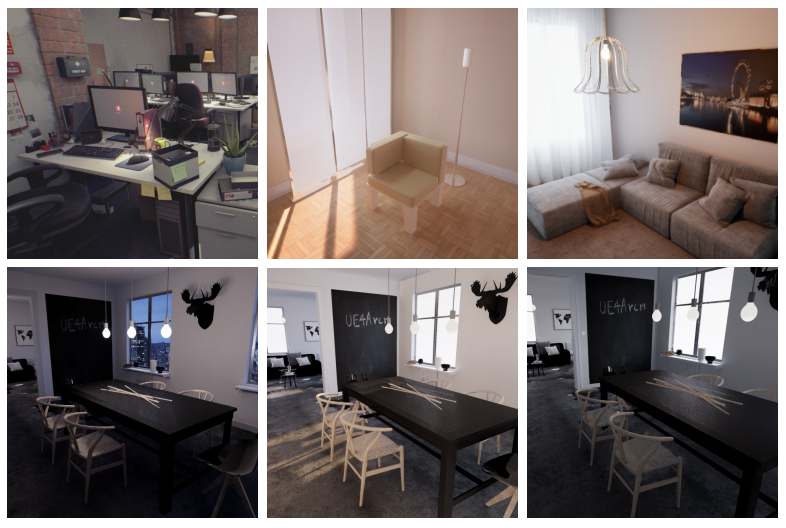
\includegraphics[width=0.7\linewidth]{archivos/robotrix}
	\caption{Snapshots of the Robotrix dataset extracted from \cite{DBLP:journals/corr/abs-1901-06514}.}
	\label{fig:robotrix}
\end{figure}

This work was motivated by a collaboration with the \gls{dtic} and the \textit{3D Perception Lab} group, which mainly focuses on the fields of 3D Computer Vision, Machine Learning and \gls{gpu} Computing. This work was carried out in the context of the COMBAHO Spanish National Project funded by \textit{Ministerio de Economia y Competitividad} of the Spanish Government and directed by Jose Garcia-Rodriguez and Miguel Angel Cazorla-Quevedo.

\section{Proposal and Goals}
\label{sec:goals}
In UnrealROX, a \gls{vr} headset is used in order to control the character or $Agent$, this means that in order to generate data an operator must manually perform the required actions for a sequence. This presents a major drawback both in time and equipment requirements.
The main proposal for this work is to develop an extension for the UnrealROX framework in order to automatize the synthetic data generation process, as well as conducting a study on how semantic segmentation architectures can transfer the knowledge of such synthetic data into the real-world domain.

As for the main objectives of this work, one of the first tasks is to establish a new type of \textit{Agent} in the framework that is not user-controlled. This would allow users to generate data sequences without the need of a \gls{vr} headset and user input, providing a faster and more convenient way to obtain datasets.

The second main objective of this work is to prove how synthetic data can be applied to real world problems. This is, in other words, use synthetically generated datasets with the intention of transfer learning to real data. In order to demonstrate this, we develop data driven algorithms and verify their effectivity with real-world datasets.

